\documentclass[aspectratio=43,11pt]{beamer}

% ============ PACKAGES ============
\usepackage[utf8]{inputenc}
\usepackage[T1]{fontenc}
\usepackage{lmodern}
\usepackage{graphicx}
\usepackage{tcolorbox}
\usepackage{booktabs}
\usepackage{fontawesome5} % Updated FontAwesome for better icon support
\usepackage{xcolor}
\usepackage{tikz}

\tcbuselibrary{skins,shadows} % Ensure these libraries are loaded correctly
\tcbuselibrary{listings,breakable} % Additional library for tcolorbox

% ============ CUSTOM COLOR PALETTE ============
\definecolor{DeepNavy}{RGB}{15,25,45}
\definecolor{NeonCyan}{RGB}{0,180,216}
\definecolor{CoralAccent}{RGB}{255,107,107}
\definecolor{LightGray}{RGB}{230,234,238}
\definecolor{AccentGold}{RGB}{255,193,7}

% ============ THEME CUSTOMIZATION ============
\usetheme{default}
\useinnertheme{rectangles}

\setbeamertemplate{navigation symbols}{}

% Custom colors
\setbeamercolor{background canvas}{bg=white}
\setbeamercolor{normal text}{fg=DeepNavy}
\setbeamercolor{frametitle}{fg=DeepNavy, bg=white}
\setbeamercolor{title}{fg=DeepNavy}
\setbeamercolor{subtitle}{fg=CoralAccent}
\setbeamercolor{item}{fg=NeonCyan}

% Custom frametitle
\setbeamertemplate{frametitle}{%
    \vspace{0.3cm}
    {\usebeamerfont{frametitle}\usebeamercolor[fg]{frametitle}\insertframetitle}
    \vspace{0.1cm}
    \textcolor{CoralAccent}{\hrule height 2pt}
    \vspace{0.2cm}
}

% Custom footer
\setbeamertemplate{footline}{%
    \hbox{%
        \begin{beamercolorbox}[wd=\paperwidth,ht=2.5ex,dp=1ex,leftskip=2ex,rightskip=2ex]{footline}
            \tiny\color{DeepNavy} EDA Project - Student Performance
            \hfill
            \insertframenumber{} / \inserttotalframenumber
        \end{beamercolorbox}
    }
}

% ============ CUSTOM TCOLORBOX STYLES ============
\tcbset{
    moderncard/.style={
        enhanced,
        colback=NeonCyan!8,
        colframe=NeonCyan,
        fonttitle=\bfseries\small,
        coltitle=white,
        colbacktitle=NeonCyan,
        boxrule=1pt,
        arc=3pt,
        left=4pt, right=4pt, top=3pt, bottom=3pt
    },
    insightbox/.style={
        enhanced,
        colback=CoralAccent!8,
        colframe=CoralAccent,
        fonttitle=\bfseries\small,
        coltitle=white,
        colbacktitle=CoralAccent,
        boxrule=1pt,
        arc=3pt,
        left=4pt, right=4pt, top=3pt, bottom=3pt
    },
    keybox/.style={
        enhanced,
        colback=AccentGold!12,
        colframe=AccentGold,
        fonttitle=\bfseries\small,
        coltitle=DeepNavy,
        colbacktitle=AccentGold,
        boxrule=1pt,
        arc=3pt,
        left=4pt, right=4pt, top=3pt, bottom=3pt
    }
}

% ============ DOCUMENT ============
\title{\textbf{Student Performance Analysis}}
\subtitle{Exploratory Data Analysis Project}
\author{Data Analytics Team}
\date{\today}

\begin{document}

% ============ SLIDE 1: TITLE ============
{
\setbeamertemplate{footline}{}
\begin{frame}[plain]
    \vspace{1.5cm}
    \begin{center}
        {\Huge\color{DeepNavy}\textbf{Student Performance}}\\[0.4cm]
        {\Large\color{CoralAccent}Exploratory Data Analysis}\\[1cm]
        
        \begin{tikzpicture}
            \node[circle, fill=NeonCyan!20, minimum size=1.5cm] at (0,0) {\color{NeonCyan}\faChartLine};
            \node[circle, fill=CoralAccent!20, minimum size=1cm] at (2,0) {\color{CoralAccent}\faUsers};
            \node[circle, fill=AccentGold!20, minimum size=1cm] at (-2,0) {\color{AccentGold}\faDatabase};
        \end{tikzpicture}
        
        \vspace{0.8cm}
        {\large\color{DeepNavy}Bachir Zekhnine \\ [0.2cm]
        Souici Mouhamed}\\
      
    \end{center}
\end{frame}
}

% ============ SLIDE 2: PROJECT OVERVIEW ============
\begin{frame}{Project Overview}
    \begin{tcolorbox}[moderncard, title=Objective]
        \small Analyze student performance to understand factors influencing academic success.
    \end{tcolorbox}
    
    \vspace{0.2cm}
    
    \begin{columns}[T]
        \column{0.48\textwidth}
        \begin{tcolorbox}[insightbox, title=Key Questions]
            \scriptsize
            \begin{itemize}\setlength{\itemsep}{1pt}
                \item Scores vary by gender?
                \item Socioeconomic impact?
                \item Test preparation effect?
            \end{itemize}
        \end{tcolorbox}
        
        \column{0.48\textwidth}
        \begin{tcolorbox}[insightbox, title=Methodology]
            \scriptsize
            \begin{itemize}\setlength{\itemsep}{1pt}
                \item Data cleaning
                \item Univariate analysis
                \item Bivariate relationships
                \item Clustering analysis
            \end{itemize}
        \end{tcolorbox}
    \end{columns}
\end{frame}

% ============ SLIDE 3: THE DATASET ============
\begin{frame}{The Dataset}
    \begin{tcolorbox}[moderncard, title=Student Performance Dataset]
        \small Academic records with demographic and socioeconomic factors
    \end{tcolorbox}
    
    \vspace{0.15cm}
    
    \begin{columns}[T]
        \column{0.48\textwidth}
        \begin{tcolorbox}[keybox, title=Dimensions]
            \centering\scriptsize
            \begin{tabular}{@{}ll@{}}
                \toprule
                \textbf{Metric} & \textbf{Value} \\
                \midrule
                Records & \textbf{1000} \\
                Features & \textbf{8} \\
                Missing & \textbf{0} \\
                \bottomrule
            \end{tabular}
        \end{tcolorbox}
        
        \column{0.48\textwidth}
        \begin{tcolorbox}[insightbox, title=Features]
            \scriptsize
            \textbf{Categorical:} Gender, Race, Parent Edu, Lunch, Test Prep
            
            \vspace{0.1cm}
            \textbf{Numerical:} Math, Reading, Writing
        \end{tcolorbox}
    \end{columns}
\end{frame}

% ============ SLIDE 4: DATA CLEANING ============
\begin{frame}{Data Cleaning Process}
    \begin{columns}[T]
        \column{0.48\textwidth}
        \begin{tcolorbox}[moderncard, title=Steps]
            \scriptsize
            \begin{enumerate}\setlength{\itemsep}{1pt}
                \item Missing values $\rightarrow$ \textbf{None}
                \item Duplicates $\rightarrow$ \textbf{Removed}
                \item Create total\_score
                \item Create average\_score
            \end{enumerate}
        \end{tcolorbox}
        
        \column{0.48\textwidth}
        \begin{tcolorbox}[insightbox, title=Results]
            \scriptsize
            \begin{itemize}\setlength{\itemsep}{1pt}
                \item Clean dataset ready
                \item New features created
                \item 1000 records retained
            \end{itemize}
        \end{tcolorbox}
    \end{columns}
    
    \vspace{0.2cm}
    
    \begin{tcolorbox}[keybox, title=Feature Engineering]
        \centering\scriptsize
        total\_score = math + reading + writing\\
        average\_score = total\_score / 3
    \end{tcolorbox}
    \end{frame}

% ============ SLIDE 5: UNIVARIATE - NUMERICAL ============
\begin{frame}{Univariate Analysis: Score Distributions}
    \begin{center}
        \includegraphics[width=0.88\textwidth, height=0.62\textheight, keepaspectratio]{images/all_scores_distribution.png}
    \end{center}
    
    \vspace{-0.15cm}
    
    \begin{tcolorbox}[insightbox, title=Insights, width=0.95\textwidth]
        \tiny
        \textbf{Math:} 66 \quad \textbf{Reading:} 69 \quad \textbf{Writing:} 68 \quad | \quad Better in reading/writing; slightly left-skewed
    \end{tcolorbox}
\end{frame}

% ============ SLIDE 6: UNIVARIATE - CATEGORICAL ============
\begin{frame}{Univariate Analysis: Categorical Variables}
    \begin{center}
        \includegraphics[width=0.88\textwidth, height=0.62\textheight, keepaspectratio]{images/gender_testprep_distribution.png}
    \end{center}
    
    \vspace{-0.15cm}
    
    \begin{tcolorbox}[insightbox, title=Distribution, width=0.95\textwidth]
        \tiny
        \textbf{Gender:} Female 51.8\% | Male 48.2\% \quad \textbf{Test Prep:} Completed 35.8\% | Not completed 64.2\%
    \end{tcolorbox}
\end{frame}

% ============ SLIDE 7: BIVARIATE - CORRELATION ============
\begin{frame}{Bivariate Analysis: Correlations}
    \begin{columns}[T]
        \column{0.5\textwidth}
        \begin{center}
            \includegraphics[width=0.9\textwidth]{images/correlation_matrix.png}
        \end{center}
        
        \column{0.48\textwidth}
        \begin{tcolorbox}[moderncard, title=Key Findings]
            \scriptsize
            \begin{itemize}\setlength{\itemsep}{1pt}
                \item \textbf{Strong} (0.95): Read-Write
                \item \textbf{Moderate} (0.82): Math-Read
                \item \textbf{Moderate} (0.80): Math-Write
            \end{itemize}
        \end{tcolorbox}
        
        \vspace{0.15cm}
        
        \begin{tcolorbox}[insightbox, title=Interpretation]
            \scriptsize
            Verbal skills are highly linked. Math is more independent.
        \end{tcolorbox}
    \end{columns}
\end{frame}

% ============ SLIDE 7b: KEY INSIGHT - TEST PREPARATION ============
\begin{frame}{Key Insight: Test Preparation Impact}
    \begin{tcolorbox}[keybox, title=\faGraduationCap\ Major Finding]
        \centering\small
        \textbf{Test prep completion improves scores across ALL subjects}
    \end{tcolorbox}
    
    \vspace{0.2cm}
    
    \begin{columns}[T]
        \column{0.48\textwidth}
        \begin{tcolorbox}[moderncard, title=Completed]
            \footnotesize
            \begin{itemize}\setlength{\itemsep}{1pt}
                \item Only \textbf{35.8\%} completed
                \item Higher Math scores
                \item Higher Reading scores
                \item Higher Writing scores
            \end{itemize}
        \end{tcolorbox}
        
        \column{0.48\textwidth}
        \begin{tcolorbox}[insightbox, title=No Course]
            \footnotesize
            \begin{itemize}\setlength{\itemsep}{1pt}
                \item \textbf{64.2\%} did not complete
                \item Lower performance
                \item Missed opportunity
                \item Need expanded access
            \end{itemize}
        \end{tcolorbox}
    \end{columns}
    
    \vspace{0.2cm}
    
    \begin{tcolorbox}[moderncard, title=Implication]
        \centering\footnotesize
        Structured support provides \textbf{tangible benefits}. Expand access to prep programs.
    \end{tcolorbox}
\end{frame}

% ============ SLIDE 7c: KEY INSIGHT - PARENTAL EDUCATION ============
\begin{frame}{Key Insight: Parental Education Correlation}
    \begin{tcolorbox}[keybox, title=\faUniversity\ Finding]
        \centering\small
        \textbf{Higher parental education = Better student performance}
    \end{tcolorbox}
    
    \vspace{0.15cm}
    
    \begin{tcolorbox}[moderncard, title=Performance Ranking]
        \centering\scriptsize
        \begin{tabular}{@{}clc@{}}
            \toprule
            \textbf{Rank} & \textbf{Parental Education} & \textbf{Performance} \\
            \midrule
            1 & Master's degree & \textcolor{green!60!black}{\textbf{Highest}} \\
            2 & Bachelor's degree & \textcolor{green!40!black}{High} \\
            3 & Associate's degree & Above Average \\
            4 & Some college & Average \\
            5 & High school & Below Average \\
            6 & Some high school & \textcolor{red!70!black}{\textbf{Lowest}} \\
            \bottomrule
        \end{tabular}
    \end{tcolorbox}
    
    \vspace{0.15cm}
    
\end{frame}

% ============ SLIDE 8: GENDER IMPACT ============
\begin{frame}{Key Trend 1: Gender Performance Gap}
    \begin{tcolorbox}[keybox, title=Finding]
        \centering\small
        \textbf{Gender influences subject-specific performance}
    \end{tcolorbox}
    
    \vspace{0.15cm}
    
    \begin{columns}[T]
        \column{0.52\textwidth}
        \begin{center}
            \includegraphics[width=0.95\textwidth]{images/gender_vs_math.png}
        \end{center}
        
        \column{0.46\textwidth}
        \begin{tcolorbox}[insightbox, title=Analysis]
            \scriptsize
            \textbf{Females:}
            \begin{itemize}\setlength{\itemsep}{0pt}
                \item Reading: +7.1 pts
                \item Writing: +9.2 pts
                \item Math: -5.2 pts
            \end{itemize}
            
            \textbf{Males:}
            \begin{itemize}\setlength{\itemsep}{0pt}
                \item Math: +5.2 pts
                \item Lower verbal scores
            \end{itemize}
        \end{tcolorbox}
    \end{columns}
\end{frame}

% ============ SLIDE 9: SOCIOECONOMIC IMPACT ============
\begin{frame}{Key Trend 2: Socioeconomic Impact}
    \begin{tcolorbox}[keybox, title=Finding]
        \centering\small
        \textbf{Lunch type (SES proxy) predicts performance}
    \end{tcolorbox}
    
    \vspace{0.15cm}
    
    \begin{columns}[T]
        \column{0.52\textwidth}
        \begin{center}
            \includegraphics[width=0.95\textwidth]{images/lunch_vs_average.png}
        \end{center}
        
        \column{0.46\textwidth}
        \begin{tcolorbox}[moderncard, title=Gap Analysis]
            \scriptsize
            \textbf{Standard vs Free/Reduced:}
            \begin{itemize}\setlength{\itemsep}{0pt}
                \item Average: \textbf{+11.1 pts}
                \item Math: +12.7 pts
                \item Reading: +11.5 pts
                \item Writing: +11.8 pts
            \end{itemize}
        \end{tcolorbox}
    \end{columns}
\end{frame}

% ============ SLIDE 9b: TOP PERFORMING GROUP ============
\begin{frame}{Key Insight: Best Performing Subgroup}
    \begin{tcolorbox}[keybox, title=Top Finding]
        \centering\small
        \textbf{Females with Standard Lunch = Highest Performers}
    \end{tcolorbox}
    
    \vspace{0.15cm}
    
    \begin{columns}[T]
        \column{0.48\textwidth}
        \begin{tcolorbox}[moderncard, title=Cross-Group Analysis]
            \scriptsize
            \textbf{By Gender \& Lunch:}
            \begin{itemize}\setlength{\itemsep}{1pt}
                \item \textcolor{green!60!black}{\textbf{Female + Standard:}} Highest
                \item Male + Standard: High
                \item Female + Free/Reduced: Moderate
                \item \textcolor{red!70!black}{Male + Free/Reduced:} Lowest
            \end{itemize}
        \end{tcolorbox}
        
        \column{0.48\textwidth}
        \begin{tcolorbox}[insightbox, title=Why This Matters]
            \scriptsize
            \begin{itemize}\setlength{\itemsep}{1pt}
                \item \textbf{Compound effect} of gender + SES
                \item Females excel in verbal skills
                \item Standard lunch = more resources
                \item Combined advantage = top scores
            \end{itemize}
        \end{tcolorbox}
    \end{columns}
    
    \vspace{0.15cm}
    
    \begin{tcolorbox}[keybox, title=Implication]
        \centering\scriptsize
        \textbf{Male students with free/reduced lunch} need the most support and intervention.
    \end{tcolorbox}
\end{frame}

% ============ SLIDE 10: CLUSTERING ============
\begin{frame}{Multivariate Analysis: Student Clusters}
    \begin{columns}[T]
        \column{0.52\textwidth}
        \begin{center}
            \includegraphics[width=0.95\textwidth]{images/clusters.png}
        \end{center}
        
        \column{0.46\textwidth}
        \begin{tcolorbox}[moderncard, title=K-Means Results]
            \scriptsize
            \textbf{3 clusters identified:}
            \begin{enumerate}\setlength{\itemsep}{0pt}
                \item High achievers (15\%)
                \item Average performers (70\%)
                \item At-risk students (15\%)
            \end{enumerate}
        \end{tcolorbox}
        
        \vspace{0.15cm}
        
        \begin{tcolorbox}[insightbox, title=Insight]
            \scriptsize
            Clear separation enables targeted interventions.
        \end{tcolorbox}
    \end{columns}
\end{frame}

% ============ SLIDE 10b: CLUSTER INSIGHTS ============
\begin{frame}{Cluster Analysis: Actionable Insights}
    \begin{tcolorbox}[keybox, title=\faUsers\ Segmentation Strategy]
        \centering\small
        \textbf{Each cluster requires different educational approaches}
    \end{tcolorbox}
    
    \vspace{0.15cm}
    
    \begin{columns}[T]
        \column{0.32\textwidth}
        \begin{tcolorbox}[moderncard, title=\faRocket\ High]
            \scriptsize
            \textbf{Profile:}
            \begin{itemize}\setlength{\itemsep}{0pt}
                \item Above-average
                \item Consistent
            \end{itemize}
            \textbf{Action:}
            \begin{itemize}\setlength{\itemsep}{0pt}
                \item Advanced programs
                \item Gifted courses
            \end{itemize}
        \end{tcolorbox}
        
        \column{0.32\textwidth}
        \begin{tcolorbox}[insightbox, title=\faBalanceScale\ Avg]
            \scriptsize
            \textbf{Profile:}
            \begin{itemize}\setlength{\itemsep}{0pt}
                \item Near mean
                \item Stable
            \end{itemize}
            \textbf{Action:}
            \begin{itemize}\setlength{\itemsep}{0pt}
                \item Maintain support
                \item Monitor
            \end{itemize}
        \end{tcolorbox}
        
        \column{0.32\textwidth}
        \begin{tcolorbox}[keybox, title=\faExclamationTriangle\ Risk]
            \scriptsize
            \textbf{Profile:}
            \begin{itemize}\setlength{\itemsep}{0pt}
                \item Below-average
                \item Needs help
            \end{itemize}
            \textbf{Action:}
            \begin{itemize}\setlength{\itemsep}{0pt}
                \item Intervention
                \item Tutoring
            \end{itemize}
        \end{tcolorbox}
    \end{columns}
\end{frame}

% ============ SLIDE 10c: STRONGEST PREDICTORS ============
\begin{frame}{Key Insight: Strongest Predictors of Success}
    \begin{tcolorbox}[keybox, title=\faSortAmountDown\ Factors Ranked]
        \centering\small
        \textbf{What matters most for student performance?}
    \end{tcolorbox}
    
    \vspace{0.2cm}
    
    \begin{tcolorbox}[moderncard, title=Impact Ranking]
        \footnotesize
        \begin{enumerate}\setlength{\itemsep}{2pt}
            \item \textbf{\textcolor{red!70!black}{Socio-economic status}} (lunch) — \textit{Strongest}
            \item \textbf{\textcolor{orange!80!black}{Test preparation}} — \textit{Strong positive effect}
            \item \textbf{\textcolor{yellow!70!black}{Parental education}} — \textit{Clear correlation}
            \item \textbf{\textcolor{green!60!black}{Race/ethnicity}} — \textit{Moderate variation}
            \item \textbf{\textcolor{blue!60!black}{Gender}} — \textit{Modest, subject-dependent}
        \end{enumerate}
    \end{tcolorbox}
    
    \vspace{0.15cm}
    
    \begin{tcolorbox}[insightbox, title=\faLightbulbO\ Critical Insight]
        \centering\scriptsize
        \textbf{Economic factors} outweigh all others — addressing socio-economic barriers is the \textbf{top priority}.
    \end{tcolorbox}
\end{frame}


% ============ SLIDE 11d: KEY TAKEAWAYS ============
\begin{frame}{Key Takeaways}
    \begin{tcolorbox}[keybox, title=\faStar\ Summary]
        \centering\small
        \textbf{What We Learned from This Analysis}
    \end{tcolorbox}
    
    \vspace{0.15cm}
    
    \begin{columns}[T]
        \column{0.48\textwidth}
        \begin{tcolorbox}[moderncard]
            \scriptsize
            \faCheckCircle\ \textbf{Socio-economic status} is the strongest predictor
            
            \vspace{0.15cm}
            \faCheckCircle\ \textbf{Test preparation} improves all scores
            
            \vspace{0.15cm}
            \faCheckCircle\ \textbf{Reading \& Writing} are linked (r=0.95)
        \end{tcolorbox}
        
        \column{0.48\textwidth}
        \begin{tcolorbox}[insightbox]
            \scriptsize
            \faCheckCircle\ \textbf{Parental education} correlates with performance
            
            \vspace{0.15cm}
            \faCheckCircle\ \textbf{Gender differences} are modest
            
            \vspace{0.15cm}
            \faCheckCircle\ \textbf{Clustering} enables interventions
        \end{tcolorbox}
    \end{columns}
    
    \vspace{0.2cm}
    
    \begin{tcolorbox}[keybox, title=\faQuoteLeft\ Bottom Line]
        \centering\scriptsize
        \textit{``Address socio-economic barriers and expand test prep access for maximum impact.''}
    \end{tcolorbox}
\end{frame}

% ============ SLIDE 12: THANK YOU ============
{
\setbeamertemplate{footline}{}
\begin{frame}[plain]
    \vspace{0.8cm}
    \begin{center}
        {\Huge\color{DeepNavy}\textbf{Thank You!}}\\[0.4cm]
        {\Large\color{CoralAccent}Questions \& Discussion}\\[0.6cm]
        
     \includegraphics[width=0.18\textwidth]{images/1736_U1RVRElPIEtBVCA0MjQtMzM.jpg}
        
        \vspace{0.4cm}
        
        \begin{tcolorbox}[moderncard, title=Contact, width=0.55\textwidth]
            \centering\scriptsize
             \faEnvelope\ mouhamed.souici@univ-bba.dz\\[0.1cm]
            \faEnvelope\ bachir.zekhnine@univ-bba.dz\\[0.1cm]
            \faGithub\ github.com/kkbbmrl/EDA
        \end{tcolorbox}
        
    \end{center}
\end{frame}
}

\end{document}
